\documentclass[11pt,a4paper]{article}
\usepackage[margin=2.2cm]{geometry}
\usepackage{adjustbox}
\usepackage{graphicx,booktabs,amsmath,amssymb,hyperref,xcolor,tikz,float,caption,subcaption,enumitem}
\usetikzlibrary{arrows.meta,positioning,fit,backgrounds}
\hypersetup{colorlinks=true,linkcolor=blue!50!black,urlcolor=blue!50!black,citecolor=blue!50!black}
\graphicspath{{../results/figures/}}
\setlist{itemsep=2pt,topsep=4pt}
\captionsetup{font=small}
\newcommand{\fit}[1]{\begin{adjustbox}{max width=\linewidth}\input{generated/#1.tex}\end{adjustbox}}

\title{\textbf{EdgeBot}\\[4pt]\large A Voice-Commanded Warehouse Mobile Manipulator:\\
Reinforcement Learning, Robotic Manipulation and Conversational AI on the Edge}
\author{Mehul Khanna\\[2pt]
UCS760 -- Edge AI and Robotics: Reinforcement Learning \& Conversational AI\\
Thapar Institute of Engineering and Technology}
\date{November 2026}

\begin{document}
\maketitle

\begin{abstract}
EdgeBot is a complete, reproducible robot software stack that a person can talk to: a spoken
command such as \emph{``move the red box from shelf A to the conveyor''} is transcribed by a
Whisper ASR model, parsed into an intent and slots by a compact BERT-style network, checked by a
dialogue manager, and executed by a JetBot-style mobile robot that navigates with a reinforcement
learning policy and manipulates objects with an inverse-kinematics-driven arm, before replying
through a neural text-to-speech voice. Each part of the UCS760 syllabus is implemented from first
principles and measured: Dynamic Programming, Monte Carlo and Temporal-Difference control on a
finite warehouse MDP; DQN and PPO in a continuous-state Gym environment with lidar and pixel
observations; DH kinematics, analytic and numerical IK, minimum-jerk trajectories and PD control for
pick-and-place and object assembly; joint intent detection and slot filling with BERT and knowledge
distillation; ASR and TTS; and ONNX/INT8 export for edge hardware. The PPO policy reaches the goal in
96\% of 300 unseen warehouse layouts, pick-and-place and three-block assembly succeed in 100/100
randomised trials, the distilled 0.5\,M-parameter NLU reaches 97.6\% frame accuracy on
sentence structures never seen in training, and the full speech loop parses 94\% of held-out spoken
commands exactly. All models run in real time on a single CPU thread.
\end{abstract}

\tableofcontents
\newpage

% =====================================================================
\section{Introduction and syllabus coverage}
Warehouse robots must move safely among shelves, handle objects precisely and accept
instructions from people who are not programmers. EdgeBot addresses all three with the techniques of
UCS760, integrated into one system rather than isolated exercises. Table~\ref{tab:syllabus} maps every
syllabus unit and laboratory to the module that implements it and the experiment that evaluates it.

\begin{table}[H]
\centering\small
\caption{Syllabus coverage.}\label{tab:syllabus}
\begin{tabular}{p{4.5cm}p{5.5cm}p{5.1cm}}
\toprule
Syllabus topic & Implementation & Evaluation \\
\midrule
MDPs, Bellman optimality, DP & \texttt{envs/warehouse\_grid.py}, \texttt{rl/tabular.py} & VI vs.\ PI on deterministic and slippery floors (\S\ref{sec:tabular}) \\
Monte Carlo, TD methods (SARSA, Q-learning, Expected SARSA, $n$-step, Double Q) & \texttt{rl/tabular.py} & 20-seed learning curves, safe vs.\ optimal routes, TD(0) prediction \\
OpenAI Gym, RL in continuous spaces, function approximation & \texttt{envs/jetbot\_nav.py} (Gymnasium API), \texttt{rl/ppo.py} & PPO with Gaussian policy, 300 unseen layouts (\S\ref{sec:nav}) \\
Deep RL, DQN, RL for vision & \texttt{rl/dqn.py}, CNN on egocentric images & Double Dueling DQN from lidar and from pixels \\
Policy gradient methods & \texttt{rl/ppo.py} (clipped surrogate, GAE) & Continuous and discrete action spaces \\
Manipulation, IK and control, gripping & \texttt{manipulation/arm.py}, \texttt{workcell.py} & IK study, tracking error (\S\ref{sec:manip}) \\
Lab: Pick-n-place, Object assembly & \texttt{Workcell.pick\_and\_place}, \texttt{Workcell.stack} & 100 randomised trials each, noise robustness \\
Task learning & \texttt{manipulation/reach\_env.py} + PPO & RL reaching vs.\ analytic IK \\
Lab: Game agent, JetBot in simulation & JetBot navigation environment & Learning curves, trajectories \\
NLP, BERT, intent slot filling, token classification & \texttt{nlu/model.py}, \texttt{nlu/bert.py}, \texttt{nlu/distill.py} & Unseen-template test, ASR-noise test (\S\ref{sec:nlu}) \\
ASR (Jasper/QuartzNet/CitriNet family) & \texttt{speech/asr.py} (Whisper, CTranslate2) & WER under noise, real-time factor (\S\ref{sec:speech}) \\
TTS (Tacotron2/WaveGlow family) & \texttt{speech/tts.py} (Piper VITS, ONNX) & Real-time factor, used for spoken replies \\
Lab: Conversational VoiceBot (JetBot commands / feedback) & \texttt{robot/agent.py}, \texttt{scripts/run\_demo.py} & End-to-end voice missions (\S\ref{sec:system}) \\
GPU computing, deployment on Jetson & \texttt{edge/export.py} (ONNX, INT8) & Latency, size, accuracy after quantisation (\S\ref{sec:edge}) \\
\bottomrule
\end{tabular}
\end{table}

% =====================================================================
\section{System architecture}\label{sec:arch}
\begin{figure}[H]
\centering
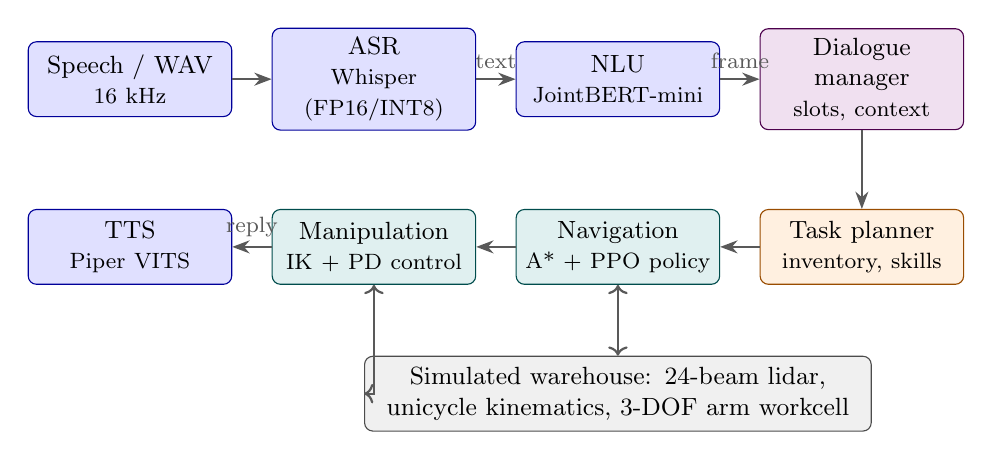
\begin{tikzpicture}[node distance=0.55cm and 0.5cm, every node/.style={font=\small},
  box/.style={draw, rounded corners=3pt, align=center, minimum height=0.95cm, text width=2.35cm, fill=#1!12, draw=#1!60!black},
  arr/.style={-{Stealth[length=2.2mm]}, thick, gray!70!black}]
\node[box=blue] (mic) {Speech / WAV\\ \footnotesize 16 kHz};
\node[box=blue, right=of mic] (asr) {ASR\\ \footnotesize Whisper (FP16/INT8)};
\node[box=blue, right=of asr] (nlu) {NLU\\ \footnotesize JointBERT-mini};
\node[box=violet, right=of nlu] (dm) {Dialogue manager\\ \footnotesize slots, context};
\node[box=orange, below=1.0cm of dm] (plan) {Task planner\\ \footnotesize inventory, skills};
\node[box=teal, left=of plan] (nav) {Navigation\\ \footnotesize A* + PPO policy};
\node[box=teal, left=of nav] (man) {Manipulation\\ \footnotesize IK + PD control};
\node[box=blue, left=of man] (tts) {TTS\\ \footnotesize Piper VITS};
\node[box=gray, below=0.9cm of nav, text width=6.2cm] (sim) {Simulated warehouse: 24-beam lidar, unicycle kinematics, 3-DOF arm workcell};
\draw[arr] (mic) -- (asr); \draw[arr] (asr) -- node[above,font=\footnotesize]{text} (nlu);
\draw[arr] (nlu) -- node[above,font=\footnotesize]{frame} (dm); \draw[arr] (dm) -- (plan);
\draw[arr] (plan) -- (nav); \draw[arr] (nav) -- (man);
\draw[arr] (man) -- node[above,font=\footnotesize]{reply} (tts);
\draw[arr, <->] (nav) -- (sim); \draw[arr, <->] (man.south) |- (sim.west);
\end{tikzpicture}
\caption{EdgeBot pipeline. Blue: conversational AI; teal: robotics; violet/orange: decision making.
The learned models (policy, NLU, TTS) are executed by ONNX Runtime; ASR by CTranslate2.}
\label{fig:arch}
\end{figure}

The robot's software is organised as a perception--decision--action loop (Fig.~\ref{fig:arch}).
Speech is transcribed, converted into a structured \emph{frame} (intent + slots), validated by the
dialogue manager against the robot's state and inventory, and compiled into skills. Navigation is
hierarchical: an A* planner over an inflated occupancy grid produces waypoints and the learned PPO
policy tracks them while reacting to obstacles through its lidar. Manipulation uses classical
kinematics and control, which are exact and verifiable for a known arm; reinforcement learning is used
for manipulation only in the task-learning study (\S\ref{sec:reach}), where it is compared against IK.

% =====================================================================
\section{Reinforcement learning foundations on a finite MDP}\label{sec:tabular}
\subsection{The warehouse grid MDP}
The robot moves on a $5\times10$ grid from the loading bay $S$ to the packing station $G$
(actions: up/right/down/left, reward $-1$ per step). Shelves block motion, and an oil spill along
the shortest route costs $-100$ and returns the robot to $S$ -- the warehouse analogue of Cliff Walking
(Sutton \& Barto, Ex.~6.6). With slip probability $p$ the intended move happens with probability
$1-p$, otherwise the robot slides perpendicular. The environment exposes its full model
$P(s',r\,|\,s,a)$ so the same MDP serves model-based and model-free methods.

\subsection{Dynamic Programming}
Value iteration applies the Bellman optimality backup
$V_{k+1}(s)=\max_a\sum_{s',r}p(s',r|s,a)\,[r+\gamma V_k(s')]$; policy iteration alternates
in-place policy evaluation with greedy improvement. Both converge to the same $V^*$ (Table~\ref{tab:dp}).
On the deterministic floor the optimal route hugs the spill (11 steps); on a slippery floor the
optimal policy moves one row away from it, trading path length for safety (Fig.~\ref{fig:dp}).
On slippery floors policy iteration needs far fewer outer iterations than value iteration (8 vs.\ 47--178 sweeps), each one more expensive.

\begin{table}[H]\centering\small\caption{Dynamic Programming on the warehouse MDP.}\label{tab:dp}
\fit{tab_dp}\end{table}
\begin{figure}[H]\centering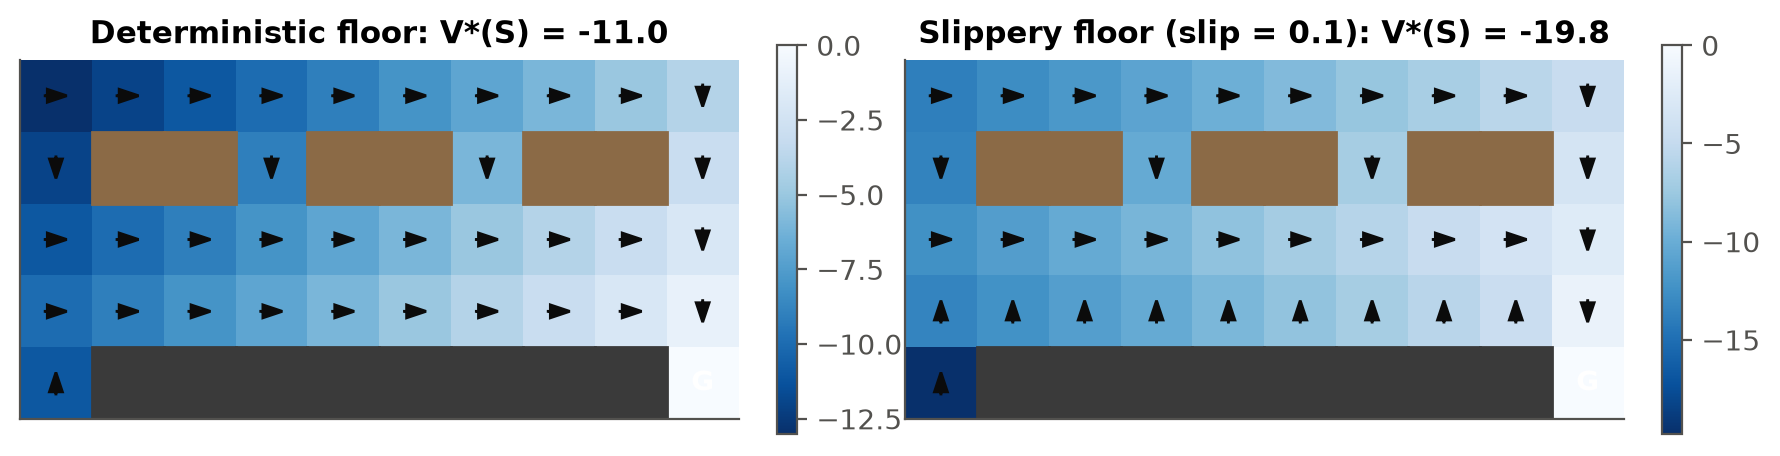
\includegraphics[width=0.95\linewidth]{dp_value_policy.png}
\caption{Optimal value function and greedy policy. Dark cells: oil spill; brown: shelves.}\label{fig:dp}\end{figure}

\subsection{Model-free control: Monte Carlo and TD}
Without the model, the agent learns from experience. Table~\ref{tab:control} and
Fig.~\ref{fig:tab} summarise 20 independent runs of each method ($\epsilon=0.1$).
\begin{itemize}
\item \textbf{Q-learning} (off-policy) learns $q_*$ and its greedy route is the optimal 11-step edge path,
but while exploring it repeatedly falls into the spill, so its online return is poor.
\item \textbf{SARSA} (on-policy) evaluates the $\epsilon$-greedy policy it actually follows, so it learns the
safest route along the far wall: higher online return, longer greedy path (17 steps). This reproduces the classic
on-/off-policy contrast of Sutton \& Barto, Fig.~6.4.
\item \textbf{Expected SARSA} removes the variance of sampling $A_{t+1}$ and gives the best online return.
\item \textbf{Double Q-learning} removes maximisation bias; \textbf{$n$-step SARSA} interpolates between TD and MC.
\item \textbf{First-visit Monte Carlo} must wait for episode termination; with $-100$ resets the returns have
high variance and it learns slowest.
\end{itemize}
\begin{table}[H]\centering\small\caption{Model-free control (20 runs, 500 episodes; MC 2000).}\label{tab:control}
\fit{tab_control}\end{table}
\begin{figure}[H]\centering
\begin{subfigure}{0.6\linewidth}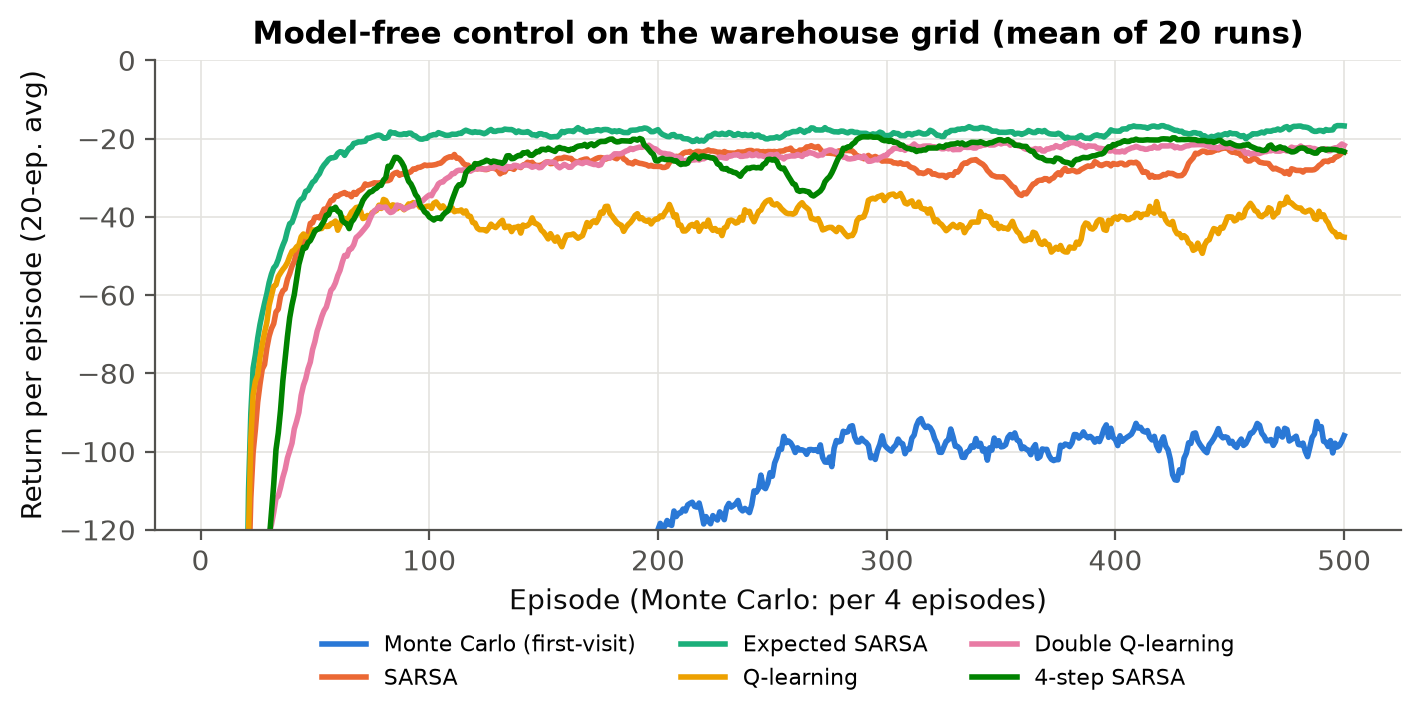
\includegraphics[width=\linewidth]{tabular_learning_curves.png}\end{subfigure}
\begin{subfigure}{0.39\linewidth}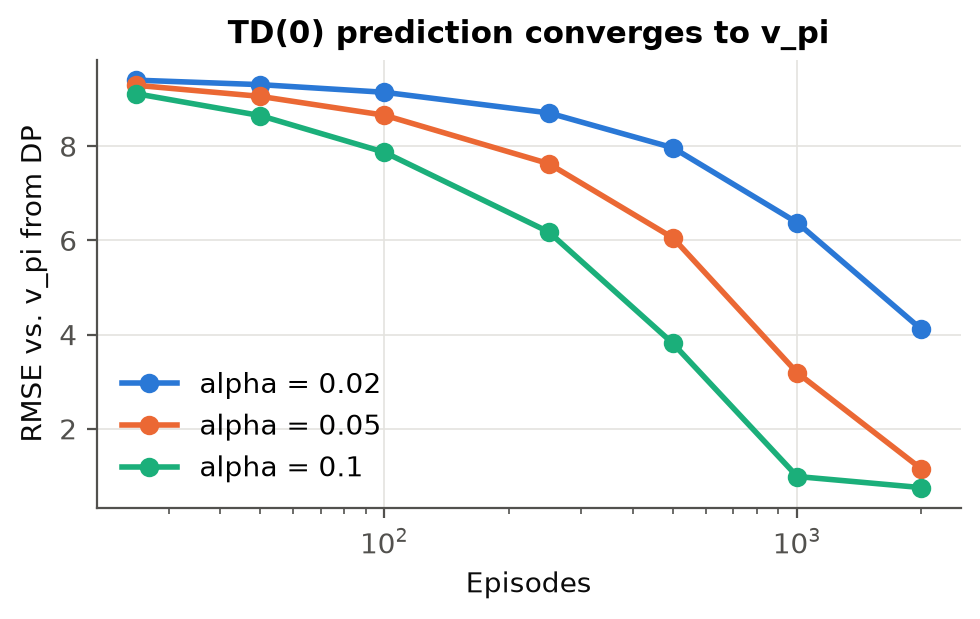
\includegraphics[width=\linewidth]{td0_prediction.png}\end{subfigure}
\caption{Left: online learning curves. Right: TD(0) prediction error w.r.t.\ $v_\pi$ computed by DP
(exploring starts, slippery floor); larger step sizes converge faster at this horizon.}\label{fig:tab}\end{figure}

% =====================================================================
\section{Deep RL for JetBot navigation in continuous space}\label{sec:nav}
\subsection{Environment}
The JetBot navigation environment follows the Gymnasium API. The robot (radius 0.12\,m) has unicycle
kinematics $\dot x=v\cos\theta,\ \dot y=v\sin\theta,\ \dot\theta=\omega$ integrated at 10\,Hz with
$v\in[0,0.5]$\,m/s, $\omega\in[-2,2]$\,rad/s. Every episode draws a new random warehouse
(0--4 shelves, 1--7 round obstacles, random start, heading and goal 1--5.5\,m apart), so the policy
must generalise rather than memorise. Observations are either
\begin{itemize}
\item \textbf{lidar}: 24 range beams over $360^\circ$ (ray--box slab test and ray--circle intersection,
vectorised), goal distance, $\sin/\cos$ of goal bearing and the previous action (29-D), or
\item \textbf{pixels}: a $2\times64\times64$ egocentric image (5\,cm/pixel occupancy + Gaussian goal marker),
rotated with the robot, for vision-based RL.
\end{itemize}
The reward is dense progress shaping $3\,(d_{t-1}-d_t)$, a step cost, an obstacle-proximity penalty
and an angular-smoothness penalty, with $+10$ on reaching the goal and $-10$ (termination) on collision.

\subsection{Algorithms}
\textbf{PPO} optimises the clipped surrogate
\[L=\mathbb{E}\big[\min(\rho_t\hat A_t,\ \mathrm{clip}(\rho_t,1\pm0.2)\,\hat A_t)\big],\qquad
\rho_t=\pi_\theta(a_t|s_t)/\pi_{\theta_{old}}(a_t|s_t),\]
with GAE($\lambda=0.95$) advantages, a diagonal Gaussian policy for continuous actions (categorical for discrete), 16 parallel
environments, early stopping on approximate KL, and bootstrapping $V(s_T)$ on time-limit truncation.
\textbf{DQN} uses experience replay, a target network, Double-DQN targets
\[y=r+\gamma\,Q_{\bar\theta}\big(s',\arg\max\nolimits_a Q_\theta(s',a)\big),\]
a dueling head and Huber loss; the pixel
version uses the Nature-DQN convolutional torso and stores images as \texttt{uint8}.

\subsection{Results}
All policies are evaluated deterministically on 300 layouts generated from seeds disjoint from training
(Table~\ref{tab:nav}). Path efficiency is the straight-line distance divided by the driven path for
successful episodes.
\begin{table}[H]\centering\small\caption{Navigation on 300 unseen layouts.}\label{tab:nav}
\fit{tab_nav}\end{table}
\begin{figure}[H]\centering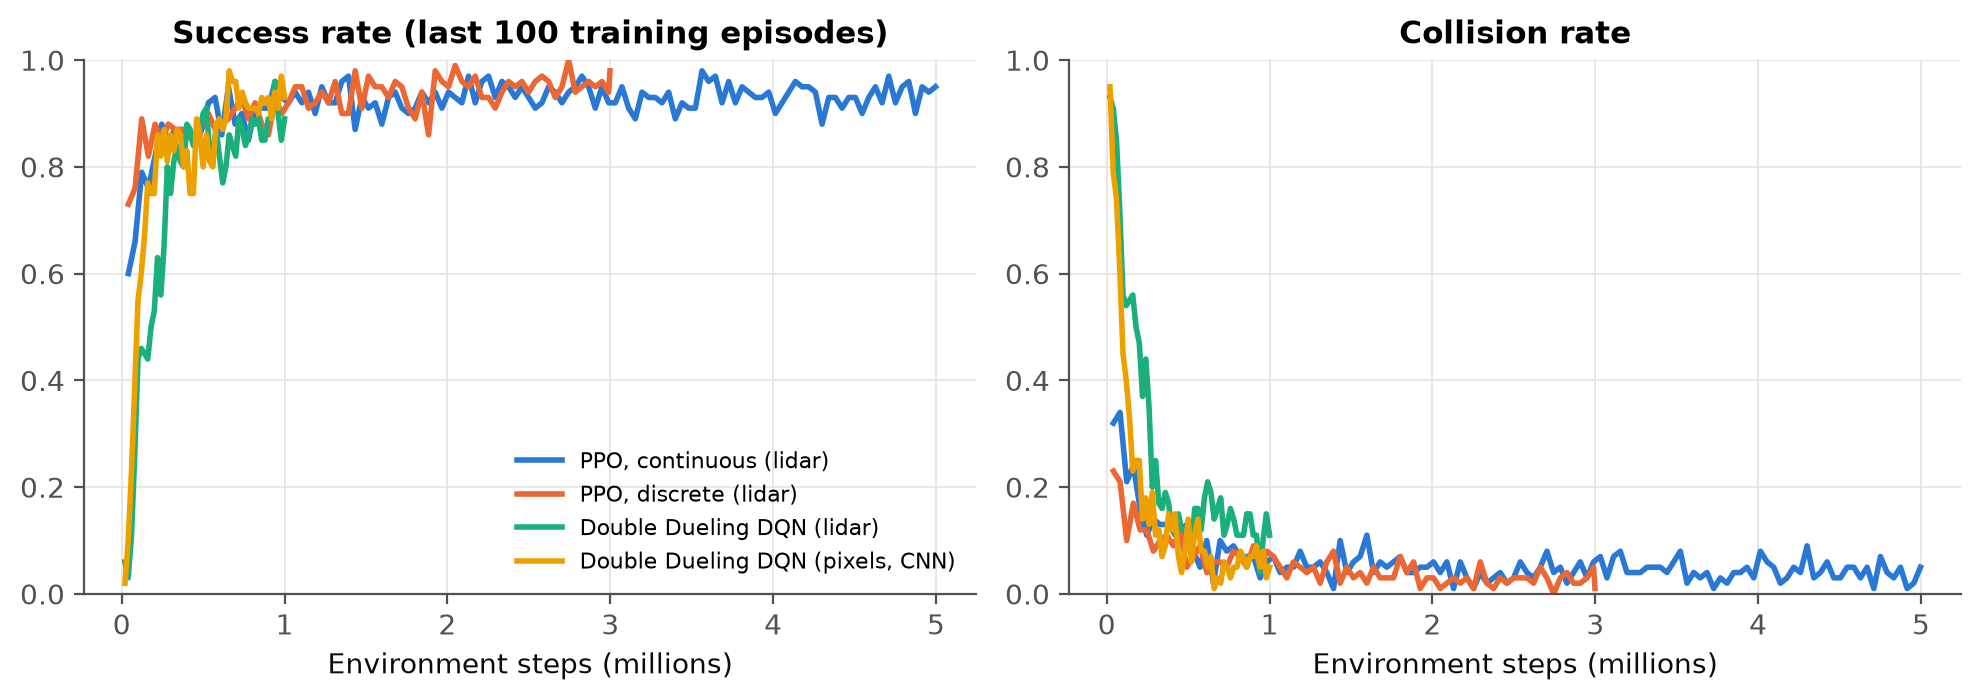
\includegraphics[width=\linewidth]{nav_learning_curves.png}
\caption{Training curves (rolling mean over the last 100 episodes).}\end{figure}
\begin{figure}[H]\centering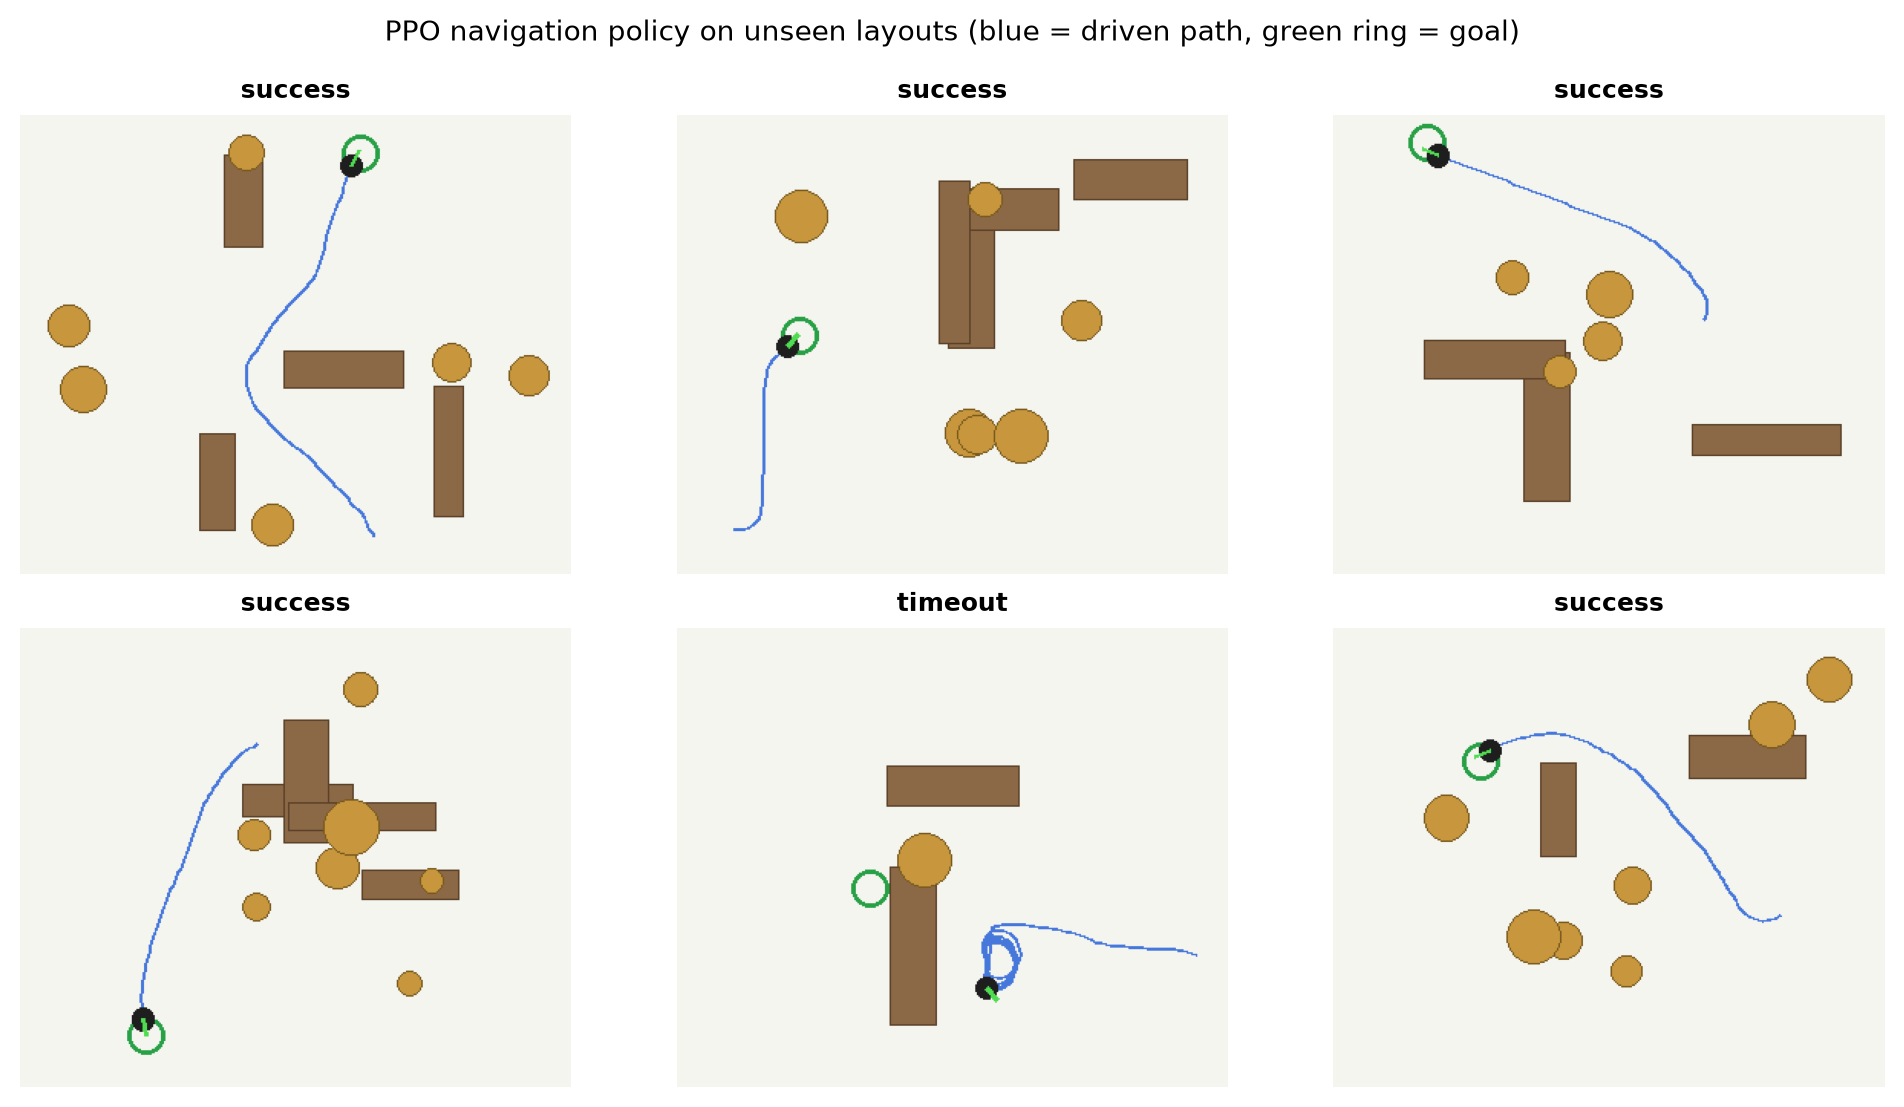
\includegraphics[width=0.9\linewidth]{nav_trajectories.png}
\caption{PPO (continuous) on unseen layouts.}\label{fig:traj}\end{figure}
Continuous-action PPO is the deployed controller: it is the most sample-efficient on CPU, produces the
smoothest motion, and its 29-D input makes the network tiny (\S\ref{sec:edge}). The pixel-based DQN
learns the same task directly from images, showing that the policy can be driven by a camera-style
representation as well.

% =====================================================================
\section{Robotic manipulation}\label{sec:manip}
\subsection{Kinematics}
The onboard arm is a planar RRR manipulator (links 0.35, 0.30, 0.12\,m) with a parallel gripper.
Forward kinematics chains standard Denavit--Hartenberg transforms
\[A_i=\mathrm{Rot}_z(\theta_i)\,\mathrm{Trans}_z(d_i)\,\mathrm{Trans}_x(a_i)\,\mathrm{Rot}_x(\alpha_i)\]
with $a=(L_1,L_2,L_3)$, $\alpha=d=0$. The end-effector pose is $(x,z,\phi)$ with $\phi=q_1+q_2+q_3$.
\textbf{Analytic IK} subtracts the wrist offset $L_3(\cos\phi,\sin\phi)$, solves the two-link
problem with the law of cosines, $\cos q_2=(w_x^2+w_z^2-L_1^2-L_2^2)/(2L_1L_2)$ (elbow-up branch), and
sets $q_3=\phi-q_1-q_2$, rejecting solutions outside joint limits. \textbf{Numerical IK} uses damped
least squares $\Delta q=J^\top(JJ^\top+\lambda^2I)^{-1}e$ on the analytic Jacobian, which is verified
against finite differences in the unit tests. Table~\ref{tab:ik} compares both; the manipulability map
$\sqrt{\det JJ^\top}$ (Fig.~\ref{fig:manip}) guided where the table slots are placed.
\begin{table}[H]\centering\small\caption{IK solvers on 2000 random reachable poses.}\label{tab:ik}
\fit{tab_ik}\end{table}
DLS is started from a fixed seed configuration, so some targets on the other elbow branch converge to
a local minimum at a joint limit; this is why the closed-form solver, which is exact and two orders of
magnitude faster, is used online, with DLS as a fallback inside Cartesian moves.

\subsection{Trajectories and control}
Free motions use quintic (minimum-jerk) joint trajectories with zero boundary velocity and
acceleration; approach and retreat use straight Cartesian lines solved point-wise by IK. Each joint is
simulated as $I\ddot q+b\dot q=\tau-g(q)$ with torque limits and a gravity model including the
payload, and is controlled by PD + acceleration feed-forward + gravity compensation. Joint tracking RMSE
stays below $0.2^\circ$ (Fig.~\ref{fig:tracking}).

\subsection{Pick-n-place and object assembly labs}
A block is grasped only if the gripper tip is within 12\,mm of its grasp point when the jaws close,
and released blocks fall onto the highest support beneath them, so success is decided by the
simulation. Pick-n-place moves a block between random table positions; assembly builds a three-block
tower in a random colour order from random start positions. Both succeed in all trials
(Table~\ref{tab:manip}). Injecting Gaussian joint-encoder noise shows no loss up to $1^\circ$, a mild drop at
$2^\circ$ and failure at $4^\circ$ (Fig.~\ref{fig:manip}), quantifying the sensing accuracy required.
\begin{table}[H]\centering\small\caption{Manipulation tasks.}\label{tab:manip}
\fit{tab_manip}\end{table}
\begin{figure}[H]\centering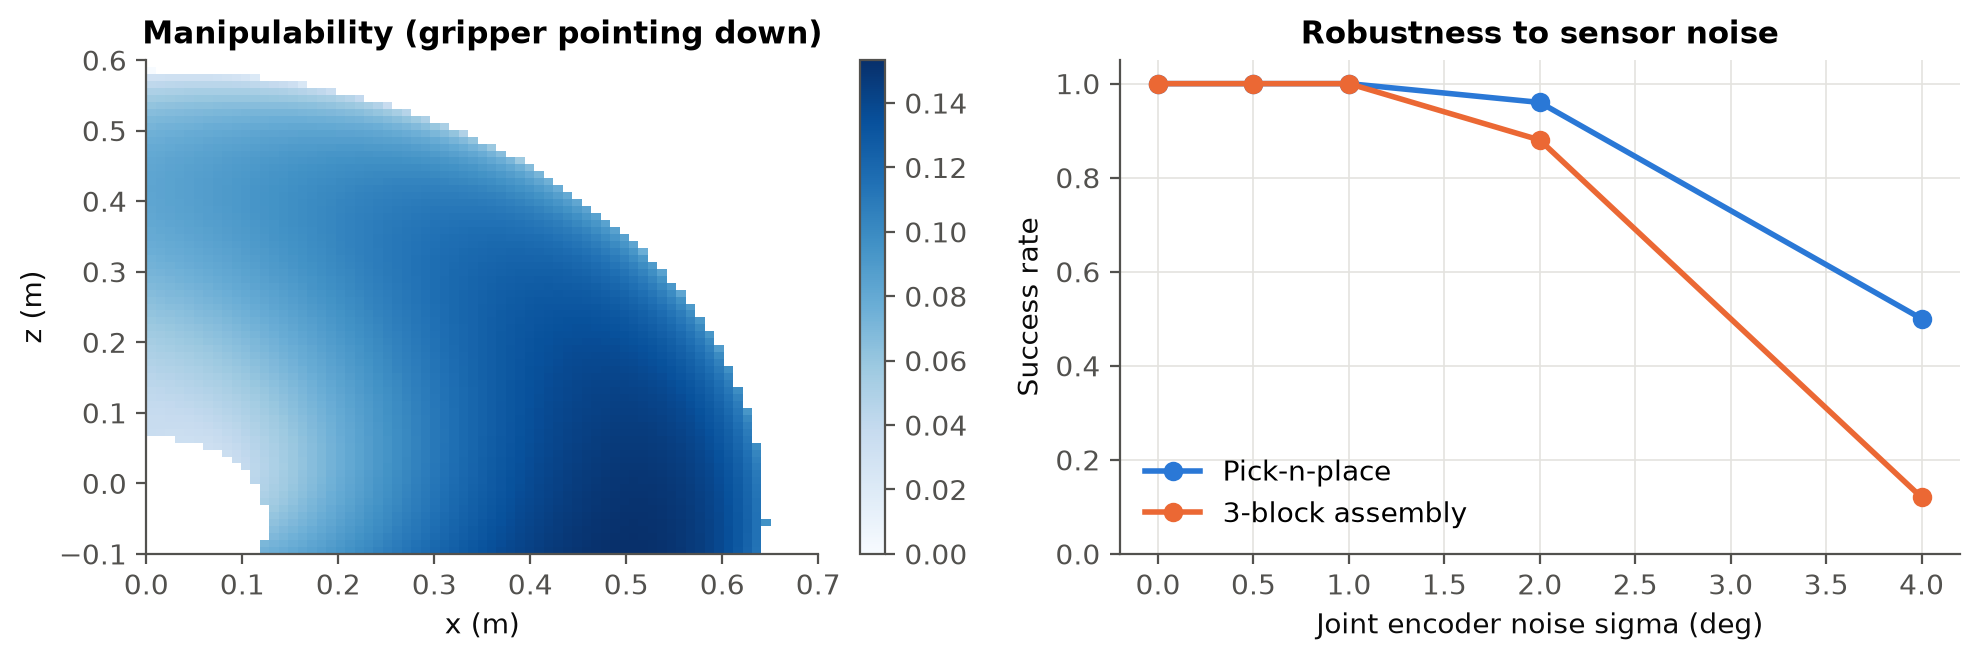
\includegraphics[width=0.95\linewidth]{manipulation_analysis.png}
\caption{Left: manipulability with a downward gripper. Right: success vs.\ encoder noise.}\label{fig:manip}\end{figure}
\begin{figure}[H]\centering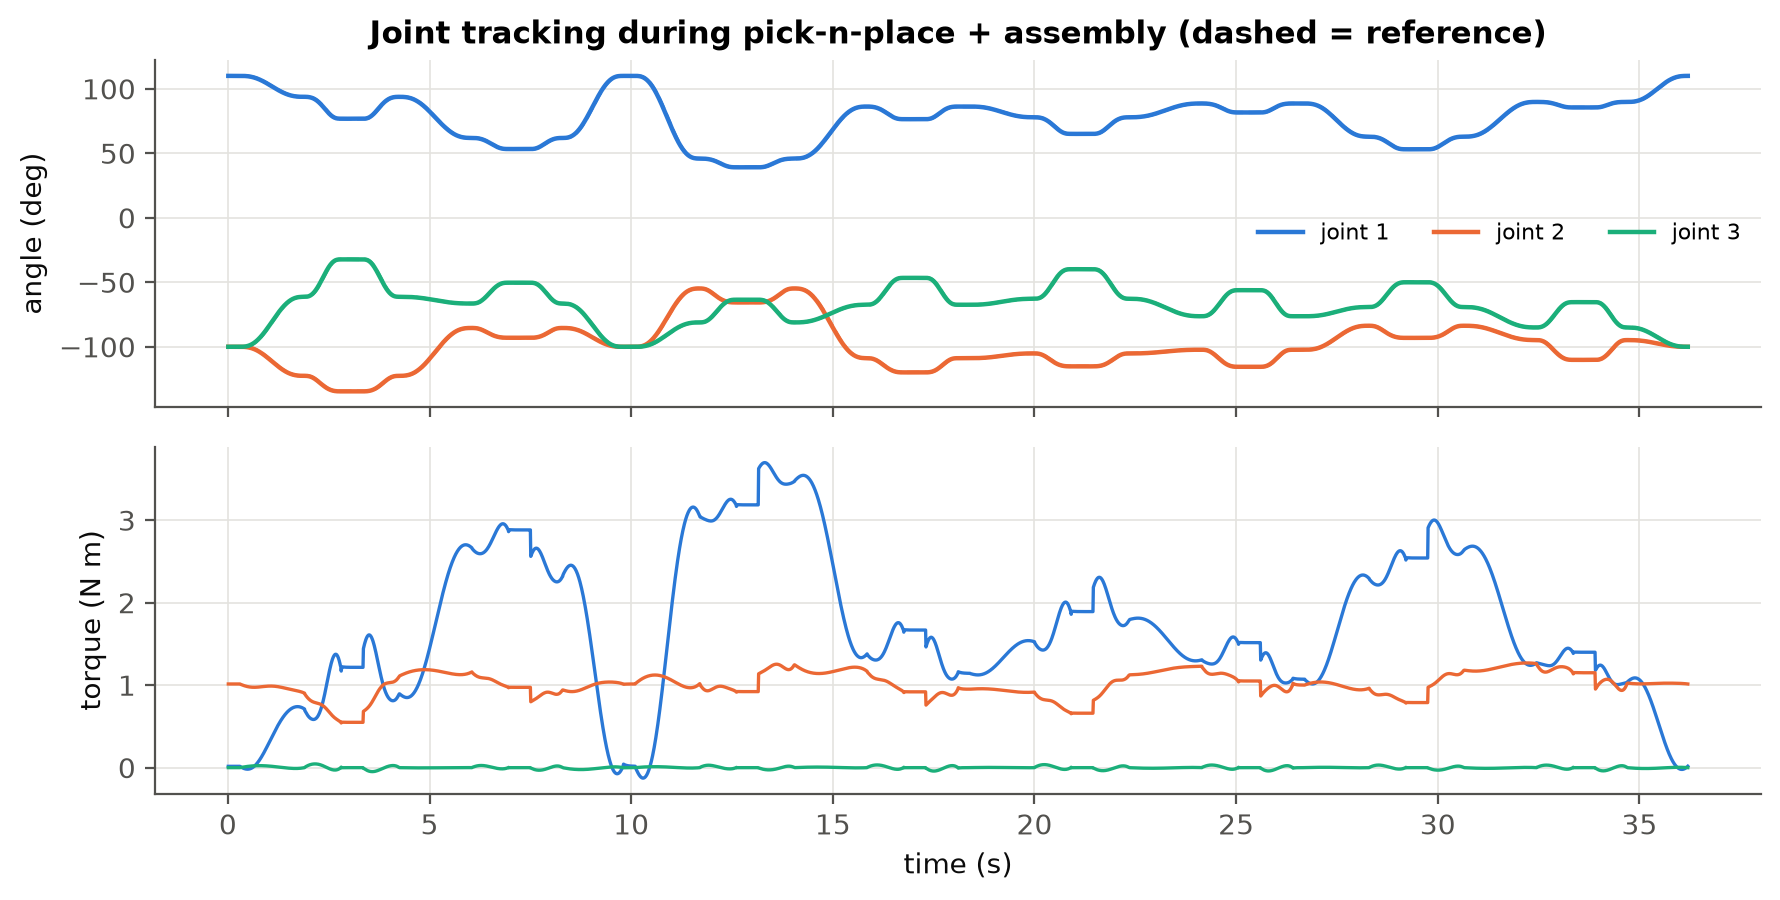
\includegraphics[width=0.85\linewidth]{joint_tracking.png}
\caption{Joint tracking and torques during pick-n-place followed by assembly.}\label{fig:tracking}\end{figure}

\subsection{Task learning with RL}\label{sec:reach}
In the reaching task the PPO agent outputs joint velocities and is rewarded for reducing the distance to
a random target with the gripper pointing down. It learns to reach within the 15\,mm tolerance in
under half a second of simulated time, but its final error remains millimetres while analytic IK is exact
(Table~\ref{tab:manip}). The comparison supports the design choice: learn what is hard to model
(navigation among unknown obstacles), compute what is known exactly (arm kinematics).

% =====================================================================
\section{Conversational AI: natural language understanding}\label{sec:nlu}
\subsection{Task and data}
Robot commands are mapped to one of nine intents (navigate, pick, place, pick\_place, stack, stop,
status, greet, help) and BIO slot tags (colour, object, source, destination) -- intent detection plus
token classification. The corpus is generated from 279 hand-written templates with six colours, seven
object types and eight locations, politeness prefixes/suffixes and an ASR-noise augmentation
(homophones such as \emph{read}/\emph{red}, \emph{self}/\emph{shelf}, dropped function words, fillers).
To measure real generalisation the templates are split \emph{before} sampling: the test set contains only
sentence structures never seen during training, once clean and once with heavy ASR noise.

\subsection{Models}
\begin{itemize}
\item \textbf{Bag-of-Words + logistic regression} -- the classical baseline (intent only).
\item \textbf{JointBERT-mini} -- a 2-layer, 4-head pre-norm Transformer encoder ($d=128$) with a learned
[CLS] token for the intent and a per-token slot head conditioned on [CLS]. Tokens are embedded as word
embedding $\oplus$ character-CNN features, so unseen or misrecognised words still get informative vectors.
\item \textbf{JointBERT (DistilBERT)} -- the pretrained 66\,M-parameter encoder fine-tuned jointly;
word labels are aligned to the first WordPiece of each word.
\item \textbf{Distilled JointBERT-mini} -- the deployed model. Following TinyBERT, the transfer set is
expanded with masked-LM augmentation (non-slot words replaced by DistilBERT's top predictions, 42\,828
new utterances), the fine-tuned teacher labels them with soft intent and slot distributions, and the
student minimises the temperature-scaled KL divergence ($T=2$) plus cross-entropy on gold labels.
\end{itemize}

\subsection{Results}
\begin{table}[H]\centering\small\caption{NLU on unseen templates (clean) and with ASR noise.}\label{tab:nlu}
\fit{tab_nlu}\end{table}
\begin{figure}[H]\centering
\begin{subfigure}{0.58\linewidth}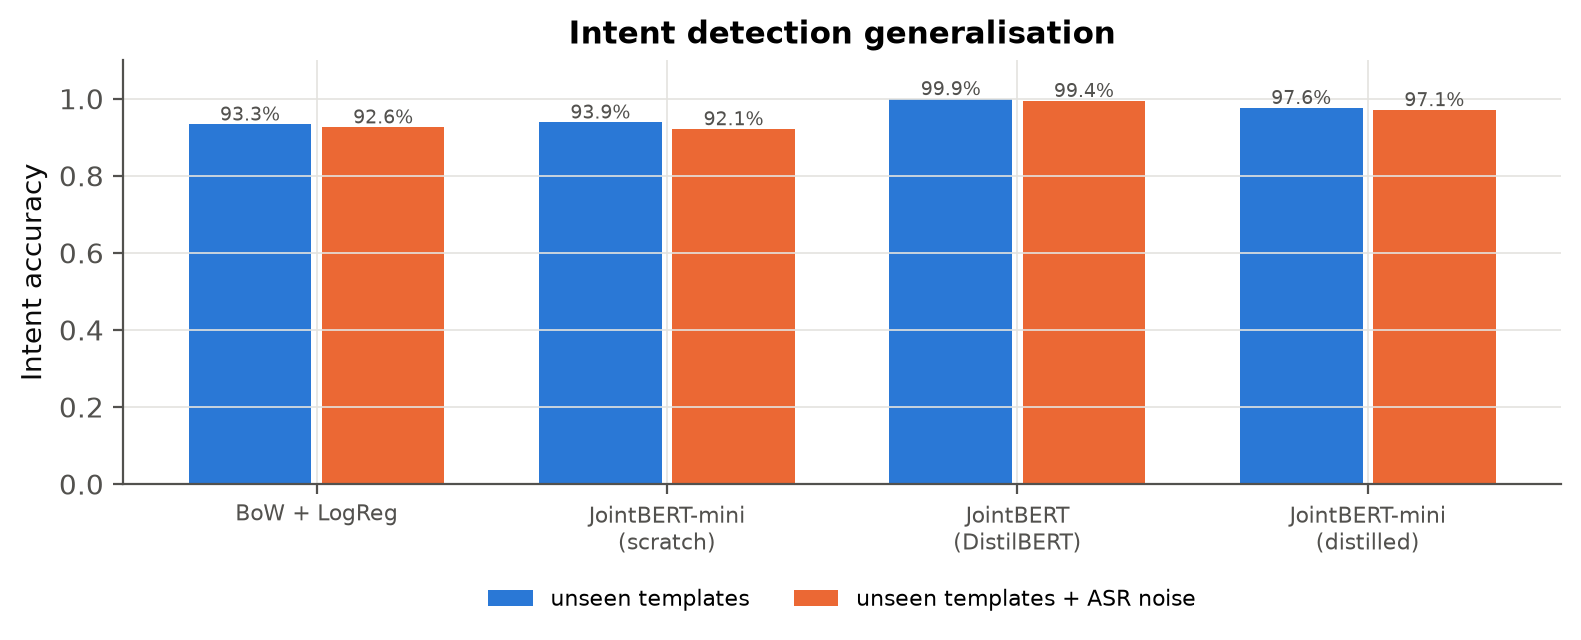
\includegraphics[width=\linewidth]{nlu_comparison.png}\end{subfigure}
\begin{subfigure}{0.41\linewidth}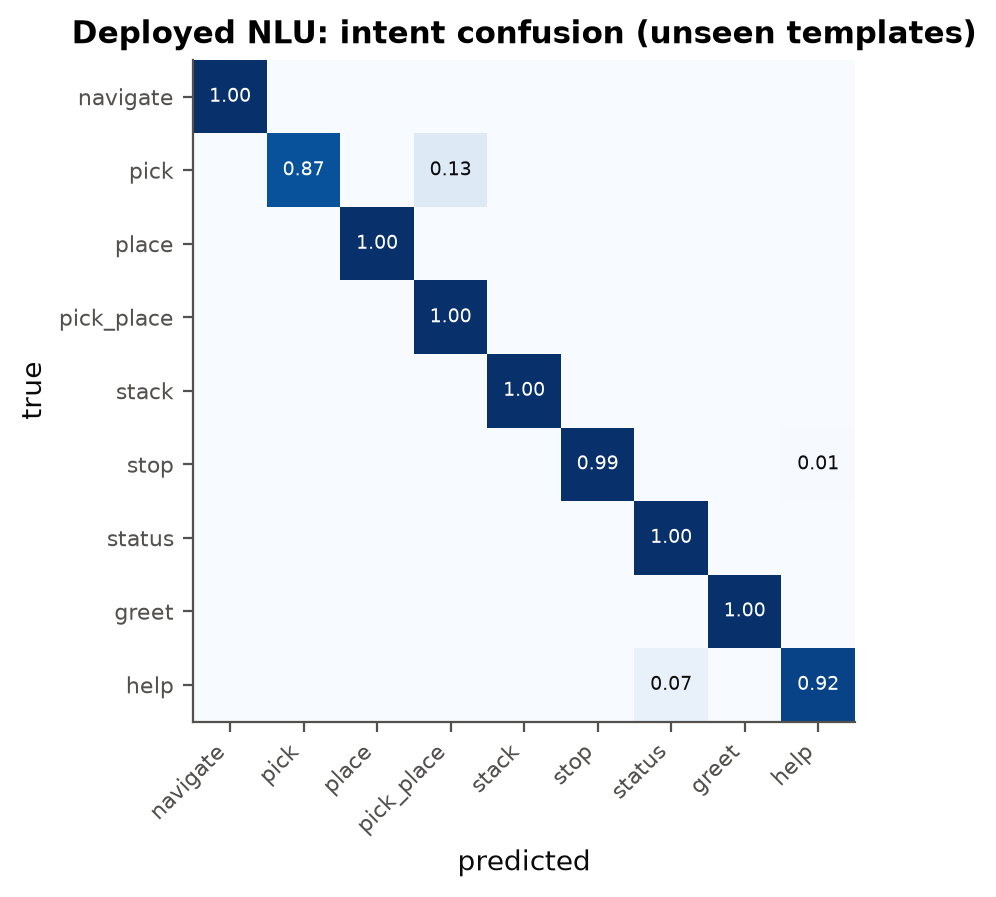
\includegraphics[width=\linewidth]{nlu_confusion.png}\end{subfigure}
\caption{Left: intent accuracy. Right: confusion matrix of the deployed model.}\end{figure}
A model trained from scratch can only match the lexical coverage of its training data, so it is barely
better than Bag-of-Words on unseen sentence structures. Pretraining supplies that knowledge: fine-tuned
DistilBERT is nearly perfect. Distillation transfers most of the gain into a network more than
100$\times$ smaller that runs in a fraction of a millisecond on one CPU core (\S\ref{sec:edge}), which is the
edge-AI trade-off in its clearest form. Slot F1 is high for every neural model because slot values
(colours, objects, locations) come from closed vocabularies; the difficulty lies in the intent.

% =====================================================================
\section{Conversational AI: speech}\label{sec:speech}
\textbf{ASR.} The syllabus covers CTC acoustic models built from 1-D convolutions -- Jasper, QuartzNet
(time--channel separable convolutions) and CitriNet (squeeze-and-excitation, subword CTC). EdgeBot uses
Whisper-base, an attention encoder--decoder trained on 680k hours, executed by CTranslate2 in FP16 on GPU
or INT8 on CPU, the same quantised-inference approach NVIDIA Riva (formerly Jarvis) uses on Jetson. A domain
prompt biases decoding toward warehouse vocabulary.

\textbf{TTS.} Tacotron2 + WaveGlow is a two-stage pipeline (autoregressive mel-spectrogram prediction,
then a flow-based vocoder). EdgeBot uses Piper, a VITS model that merges both stages into one
non-autoregressive network exported to ONNX, which suits embedded CPUs.

\textbf{End-to-end evaluation.} 150 held-out commands are spoken by the TTS voice, optionally corrupted
with white noise, transcribed and parsed. Slot values are compared after canonicalisation, so a
recognised \emph{``shelf B''} matches the gold \emph{``shelf b''}. The speech is synthetic, which makes
this an optimistic test of acoustic robustness (one speaker, studio-clean), but a strict test of the
language side, because every utterance uses unseen sentence templates.
\begin{table}[H]\centering\small\caption{Speech-to-frame accuracy (150 held-out commands).}\label{tab:voice}
\fit{tab_voice}\end{table}
\begin{table}[H]\centering\small\caption{Speech model throughput (RTF = processing time / audio duration).}
\fit{tab_speech_rtf}\end{table}

% =====================================================================
\section{Edge deployment}\label{sec:edge}
GPUs execute thousands of threads in SIMT warps; their advantage appears with large batches or large
models (ASR, BERT training), while a robot controller runs batch-1 inference on small networks, where
CPU latency, memory and energy dominate. All learned controllers are therefore exported to ONNX
(opset 17, dynamic batch/sequence axes), verified against PyTorch, and quantised with dynamic INT8
(weights quantised per tensor, activations at run time, no calibration data). ONNX is the input format
of TensorRT on Jetson (\texttt{trtexec --onnx=model.onnx --fp16}) and runs unchanged under ONNX Runtime
on ARM CPUs. Latencies in Table~\ref{tab:edge} are medians of 300 batch-1 calls on a single CPU thread
of the development laptop (CUDA: RTX 4050 Laptop GPU); they were not measured on Jetson hardware.
\begin{table}[H]\centering\small\caption{Model size and batch-1 latency.}\label{tab:edge}
\fit{tab_edge}\end{table}
\begin{table}[H]\centering\small\caption{Task metrics after export and quantisation.}\label{tab:quant}
\fit{tab_quant}\end{table}
\begin{figure}[H]\centering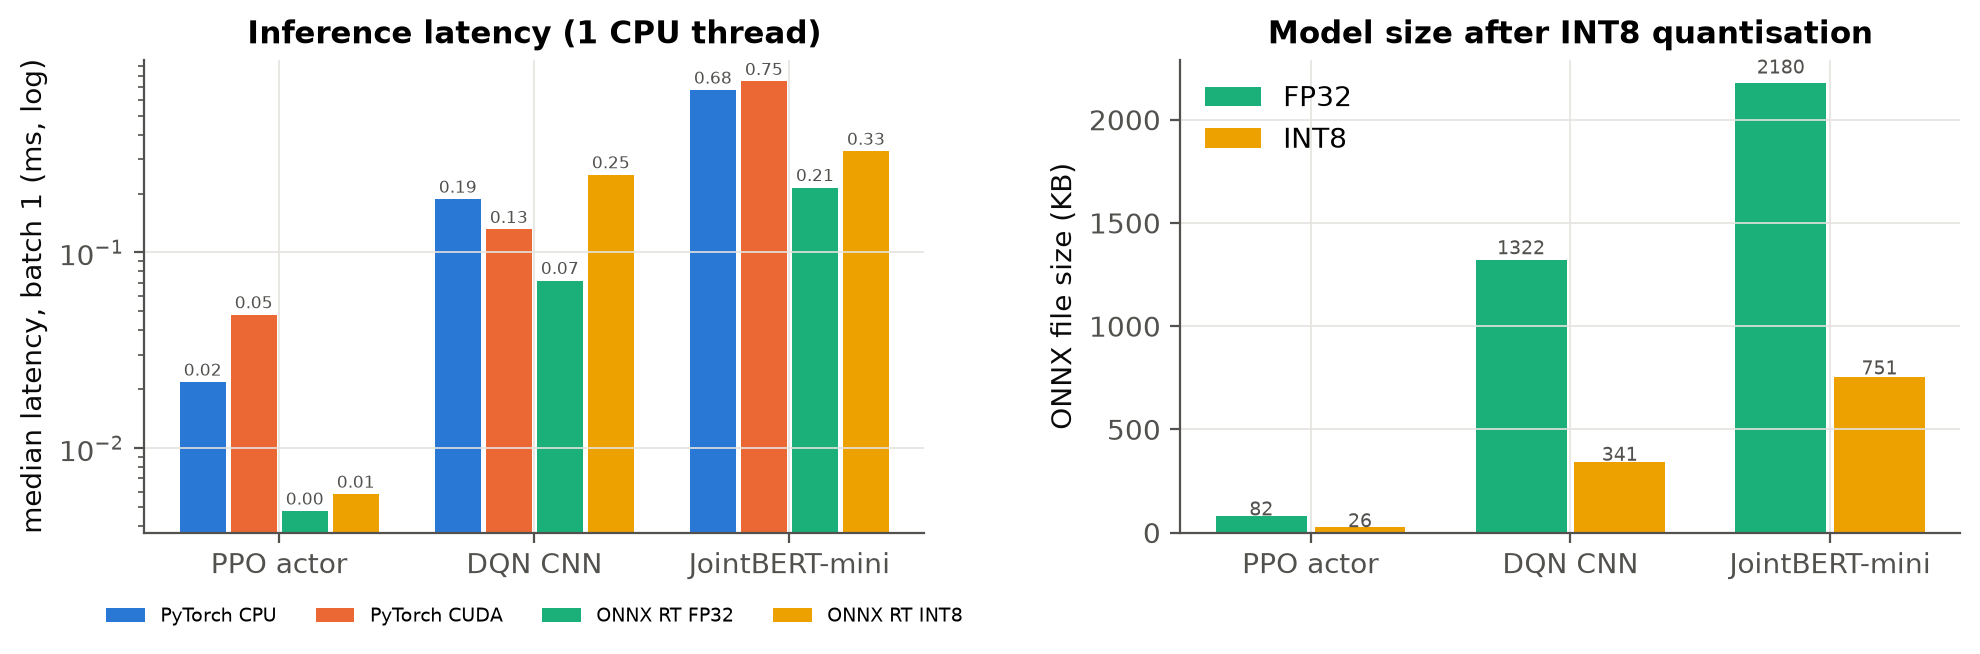
\includegraphics[width=\linewidth]{edge_benchmark.png}
\caption{Latency (log scale) and model size.}\end{figure}
For these small networks the GPU gives little or no benefit at batch 1, because kernel-launch and transfer
overheads dominate the arithmetic: it is slower than the CPU for the MLP policy and slower than ONNX Runtime
on one CPU thread for every model. ONNX Runtime beats eager PyTorch through graph optimisation and
lower per-call overhead. Dynamic INT8 shrinks the models 3--4$\times$; on this x86 CPU it does not reduce
latency for such small matrices, because activations are quantised on every call -- its benefit here is
memory footprint. For the PPO actor and the NLU, accuracy is preserved (Table~\ref{tab:quant}).

\textbf{Quantisation study (vision policy).} The pixel-based DQN is more sensitive: a greedy policy picks
the action with the largest Q-value, and the gaps between Q-values are small compared with per-tensor
INT8 error in the convolutions. Table~\ref{tab:dqnq} shows the standard remedies in order: per-channel
weight scales recover a large part of the loss, and static quantisation in QDQ format with activation
ranges calibrated on 1\,167 real observations recovers most of the rest while also being the fastest
variant. QDQ graphs with calibrated scales are exactly what TensorRT consumes for INT8 on Jetson.
\begin{table}[H]\centering\small\caption{INT8 quantisation of the pixel-based DQN (100 unseen layouts).}\label{tab:dqnq}
\fit{tab_dqn_quant}\end{table}

% =====================================================================
\section{Integrated system demonstration}\label{sec:system}
\texttt{scripts/run\_demo.py --voice} runs a scripted eight-turn conversation through the complete
stack with ONNX Runtime models: greeting; \emph{``move the red box from shelf A to the conveyor''}
(navigate, pick, navigate, place); an under-specified \emph{``pick up the box''}, which triggers the
clarification question \emph{``Which colour item should I pick up?''} and is completed by \emph{``the blue
one''}; \emph{``put it on the packing station''}, where \emph{it} is resolved to the carried crate; a
three-block tower at the workbench; a status report; and return to the charging dock. Each command is
synthesised to speech and passed through ASR, so the full voice loop runs without a microphone; with
\texttt{--mic} it runs live. The run is rendered to \texttt{results/media/edgebot\_demo.mp4}, showing the
A* plan, the PPO trajectory and lidar beams next to the arm workcell and the dialogue, and the robot's
spoken replies are written to WAV files.

The dialogue manager rejects low-confidence parses (asks the user to rephrase), checks the inventory
before acting (\emph{``I could not find a purple tote on the shelf A''}), refuses to pick while carrying,
and reports navigation or grasp failures instead of claiming success.

% =====================================================================
\section{Limitations and future work}
\begin{itemize}
\item The simulator is 2-D: navigation uses ideal unicycle kinematics and noise-free lidar, and the arm
moves in a vertical plane. Sim-to-real transfer to a physical JetBot would need sensor noise, latency and
domain randomisation, and a 6-DOF arm would need orientation IK.
\item Speech tests use one synthetic voice; real users, accents and far-field microphones will raise WER.
\item The NLU corpus is template-generated; collecting real user commands would give a more realistic test.
\item Latency was measured on a laptop CPU/GPU. Running \texttt{trtexec} on a Jetson Orin Nano with the
exported ONNX files is the natural next step.
\end{itemize}

% =====================================================================
\section{Reproducibility}
Every number in this report is produced by a script in the repository and stored as JSON in
\texttt{results/}; the tables above are generated from those files by \texttt{scripts/build\_tables.py}.
\texttt{make all} re-runs every experiment, figure, table and this document; \texttt{pytest} runs 18 unit tests
covering the MDP model, DP/TD algorithms, lidar geometry, collisions, path planning, FK/IK/Jacobian,
trajectories, pick-and-place, assembly, NLU data and span decoding and the dialogue manager.

\section*{References}
\small
\begin{enumerate}[leftmargin=*]
\item R.~S.~Sutton and A.~G.~Barto, \emph{Reinforcement Learning: An Introduction}, 2nd ed., MIT Press, 2018.
\item M.~Wiering and M.~van Otterlo (eds.), \emph{Reinforcement Learning: State of the Art}, Springer, 2012.
\item S.~Russell and P.~Norvig, \emph{Artificial Intelligence: A Modern Approach}, Pearson, 2016.
\item D.~Jurafsky and J.~H.~Martin, \emph{Speech and Language Processing}, 3rd ed.\ draft, 2019.
\item I.~Goodfellow, Y.~Bengio and A.~Courville, \emph{Deep Learning}, MIT Press, 2016.
\item V.~Mnih et al., ``Human-level control through deep reinforcement learning,'' \emph{Nature}, 2015.
\item H.~van Hasselt, A.~Guez and D.~Silver, ``Deep reinforcement learning with double Q-learning,'' AAAI, 2016.
\item Z.~Wang et al., ``Dueling network architectures for deep reinforcement learning,'' ICML, 2016.
\item J.~Schulman et al., ``Proximal policy optimization algorithms,'' arXiv:1707.06347, 2017.
\item J.~Schulman et al., ``High-dimensional continuous control using generalized advantage estimation,'' ICLR, 2016.
\item J.~Devlin et al., ``BERT: Pre-training of deep bidirectional transformers,'' NAACL, 2019.
\item V.~Sanh et al., ``DistilBERT, a distilled version of BERT,'' arXiv:1910.01108, 2019.
\item Q.~Chen, Z.~Zhuo and W.~Wang, ``BERT for joint intent classification and slot filling,'' arXiv:1902.10909, 2019.
\item X.~Jiao et al., ``TinyBERT: Distilling BERT for natural language understanding,'' Findings of EMNLP, 2020.
\item A.~Radford et al., ``Robust speech recognition via large-scale weak supervision (Whisper),'' ICML, 2023.
\item S.~Kriman et al., ``QuartzNet: Deep automatic speech recognition with 1D time-channel separable convolutions,'' ICASSP, 2020.
\item J.~Shen et al., ``Natural TTS synthesis by conditioning WaveNet on mel spectrogram predictions (Tacotron 2),'' ICASSP, 2018.
\item J.~Kim, J.~Kong and J.~Son, ``Conditional variational autoencoder with adversarial learning for end-to-end text-to-speech (VITS),'' ICML, 2021.
\item T.~Yoshikawa, ``Manipulability of robotic mechanisms,'' \emph{IJRR}, 1985.
\item M.~W.~Spong, S.~Hutchinson and M.~Vidyasagar, \emph{Robot Modeling and Control}, Wiley, 2006.
\end{enumerate}
\end{document}
